\ifdefined\USERMANUAL
  \newcommand{\doctype}{PODRĘCZNIK UŻYTKOWNIKA}
\else
  \newcommand{\doctype}{KARTY REFERENCYJNE}
\fi

\maketitlepage{TAIPO}{Rozszerzenie MIDI}{TAIPO_SILVER_cutout_small_2}{\doctype}

\newpage
\tableofcontents
\newpage
\part{Przegląd}
\newpage
\section{Przegląd}\label{section:installation}
\subsection{Przegląd}
\paragraph*{}
\textbf{TAIPO} Rozszerzenie MIDI umożliwia bezproblemowe połączenie The Centre z zewnętrznym sprzętem, w tym z komputerami, za pomocą standardowego kabla MIDI TRS typu B.
\subsection{Zawartość opakowania}
\paragraph*{}
Pakiet \textbf{TAIPO} zawiera następujące akcesoria:
\begin{enumerate}
  \item Moduł Eurorack \textbf{TAIPO}
  \item Standardowy kabel zasilający Eurorack (10-pin do 16-pin)
  \item Kabel MIDI-EX do połączenia z \textbf{The Centre}
\end{enumerate}

\newpage
\part{Instalacja}
\newpage
\section{Instalacja}
\subsection{Kroki instalacji}
\paragraph*{}
Instalacja modułu \textbf{TAIPO} przebiega zgodnie ze standardową procedurą instalacji dowolnego modułu Eurorack w obudowie użytkownika.

\begin{figure}[h]
  \centering
  \includegraphics[height=0.5\linewidth]{taipo_the_centre_cable_install.jpg}
  \includegraphics[height=0.5\linewidth]{taipo_cable_install.jpg}
  \caption{Instalacja kabla na obu końcach}
  \label{fig:midsinglenote}
\end{figure}

\subsection{Ważne uwagi dotyczące instalacji}
\paragraph*{}
Upewnij się, że kabel jest prawidłowo zorientowany podczas instalacji. Kolejność kolorów po stronie The Centre powinna być następująca: \textbf{CZARNY, CZERWONY, ŻÓŁTY, ZIELONY} od góry, natomiast po stronie TAIPO odwrotnie: \textbf{ZIELONY, ŻÓŁTY, CZERWONY, CZARNY}.
\newline$\blacksquare$ \textbf{Ważne}: Po stronie The Centre podłącz kabel do złącza MIDI-EX, jak pokazano na powyższym rysunku. Drugie złącze jest przeznaczone do przesyłania sygnału MIDI z The Centre do TWINS.

\newpage
\part{MIDI}
\newpage
\section{Typy kabli MIDI}
\subsection{Typ kabla TAIPO}
\paragraph*{}
Moduł \textbf{TAIPO} wykorzystuje kabel MIDI 3,5 mm TRS (Tip-Ring-Sleeve) typu B. Zobacz: \underline{\nameref{section:cabletypeb}}
\subsection{O sygnale MIDI}
\paragraph*{}
Sygnał MIDI jest przesyłany przez kabel MIDI przy użyciu protokołu RS-232 z niestandardową prędkością 31 250 bodów (bitów na sekundę). Połączenia MIDI są kierunkowe, co oznacza, że wewnętrzna konfiguracja pinów w kablu ma znaczenie, ponieważ prąd płynie w jednym kierunku. O ile standardowe kable MIDI DIN nie sprawiają problemów, kable 3,5 mm TRS mogą się różnić z powodu braku początkowo zdefiniowanego standardu, co doprowadziło do powstania różnych konfiguracji okablowania. W rezultacie pojawiło się kilka standardów.
\newline$\blacksquare$ \textbf{Uwaga}: Różne standardy TRS nie są wzajemnie zamienne ani kompatybilne. Aby połączyć urządzenia z różnymi standardami TRS, należy użyć odpowiedniego kabla.
\subsection{Złącze DIN}
Standardowy kabel MIDI wykorzystuje 5-pinowe złącze DIN, zapewniające niezawodne połączenie.
\subsection{Typy złączy TRS}
\subsubsection{Złącze typu A}
Złącze TRS typu A określa \textbf{TIP} wtyczki 3,5 mm jako \textit{\textbf{źródło}}, a \textbf{RING} jako \textit{\textbf{odbiornik}}.
\newline
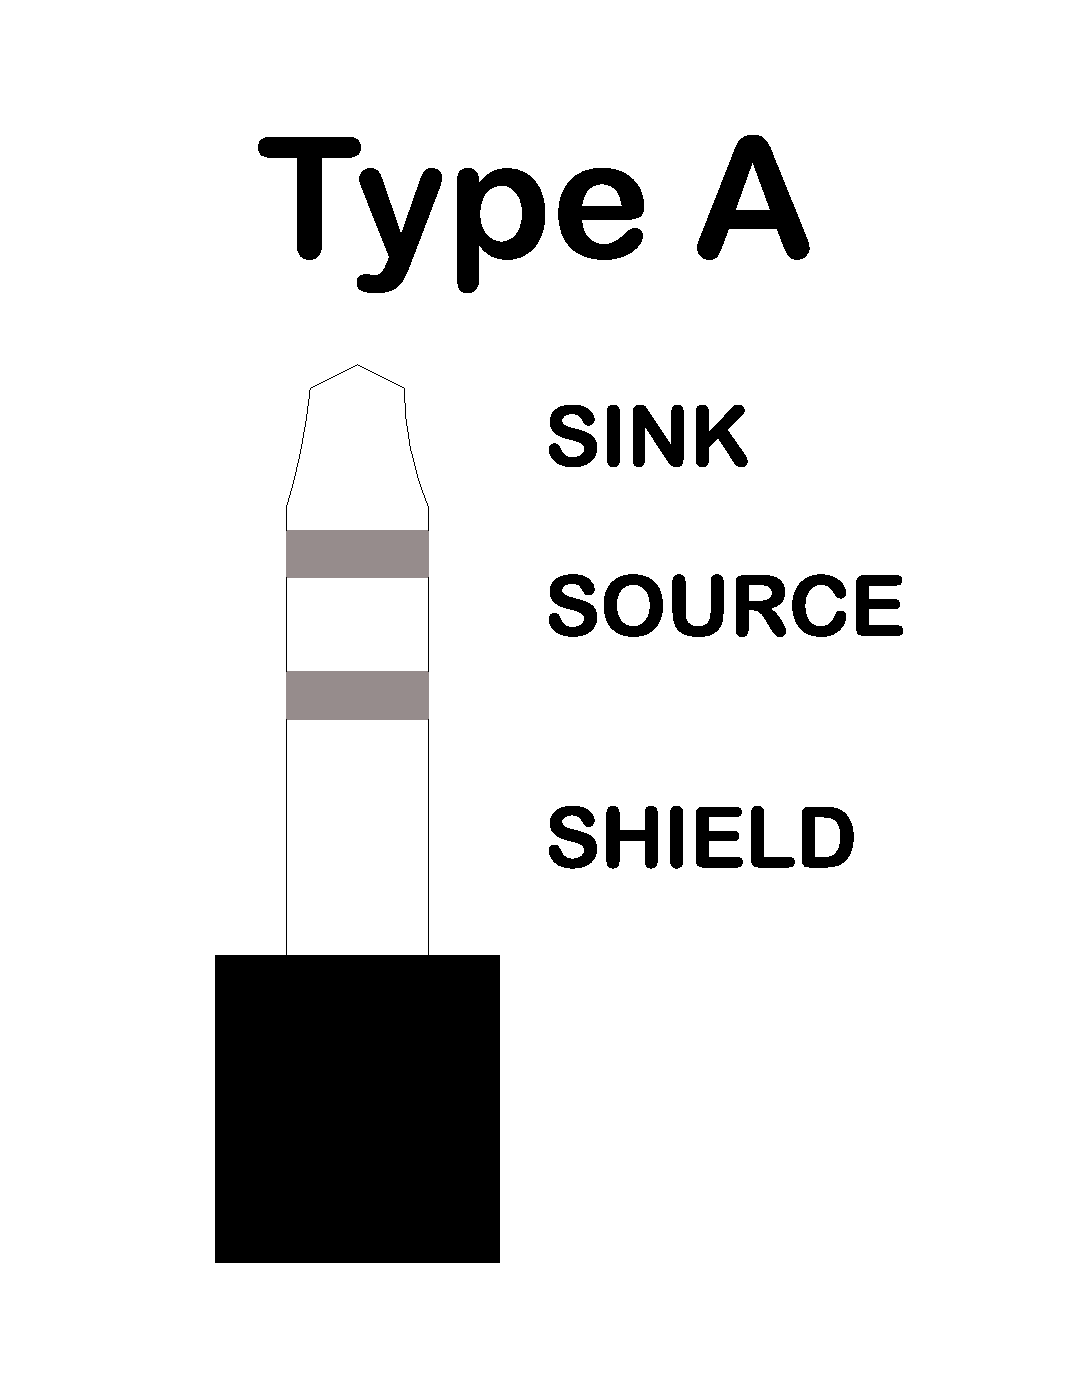
\includegraphics[height=0.3\linewidth]{midi_trs_type_a.eps}
\newline$\bigstar$ Marki używające typu A: Korg, Akai
\subsubsection{Złącze typu B}\label{section:cabletypeb}
Złącze TRS typu B określa \textbf{TIP} wtyczki 3,5 mm jako \textit{\textbf{odbiornik}}, a \textbf{RING} jako \textit{\textbf{źródło}}.
\newline$\blacksquare$ Typ B jest powszechnie stosowany w środowisku modularnym Eurorack.
\newline
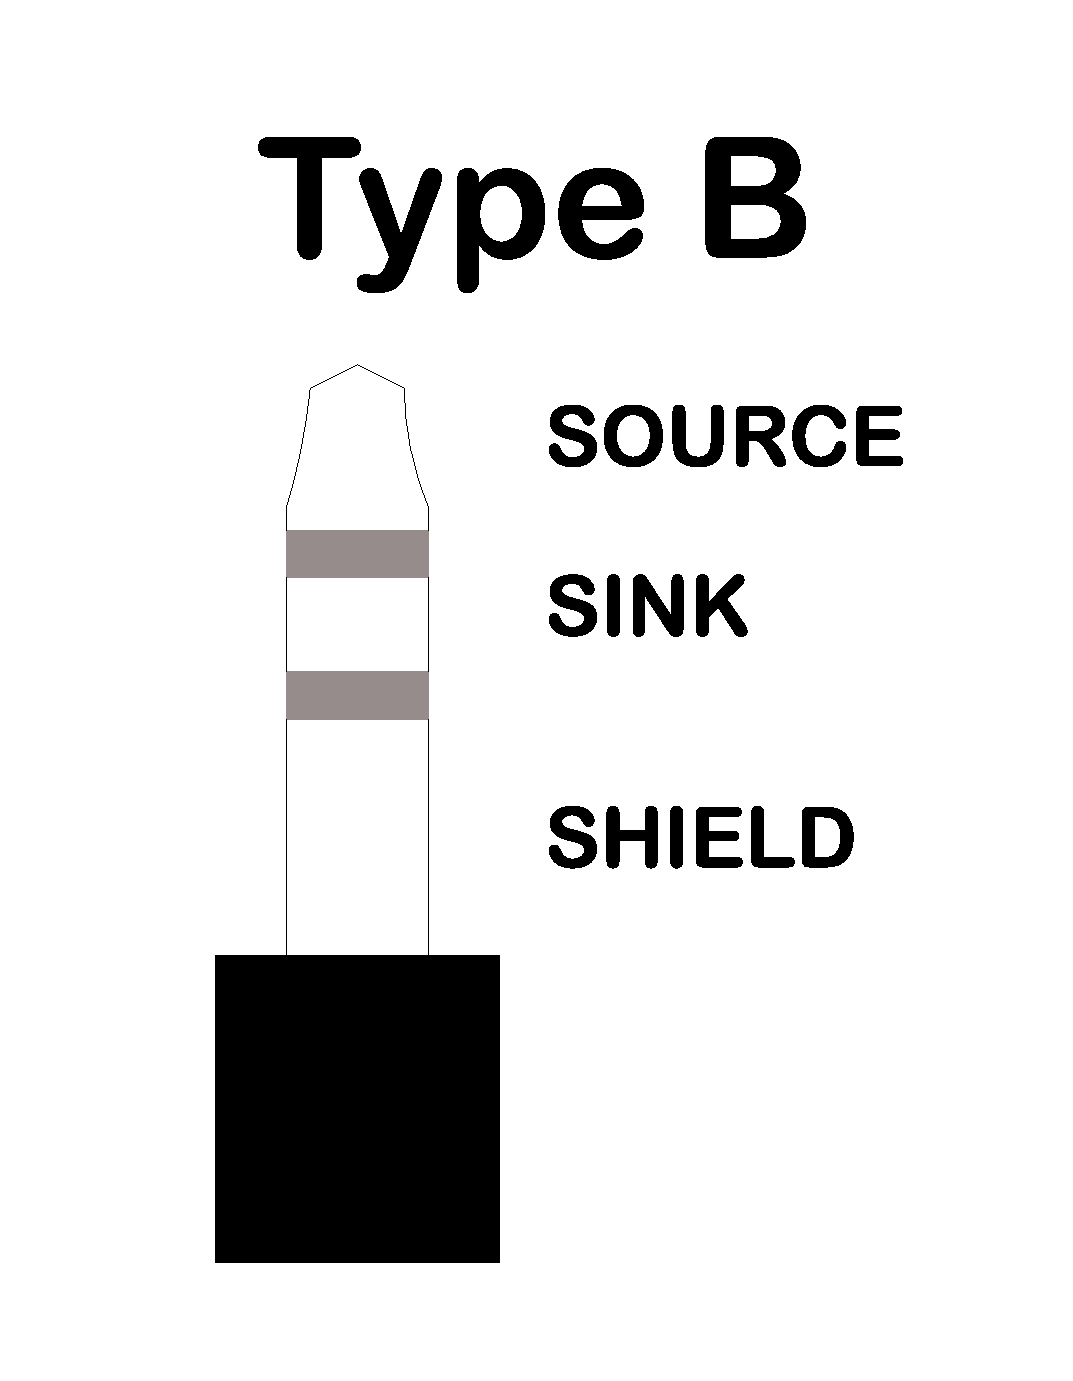
\includegraphics[height=0.3\linewidth]{midi_trs_type_b.eps}
\newline$\bigstar$ Marki używające typu B: Arturia, Novation, 1010 Music